%%%%%%%%%%%%%%%%%%%%%%%%%%%%%%%%%%%%%%%%%%%%%%%%%%%%%%%%%%%%%%%
%
% Welcome to Overleaf --- just edit your LaTeX on the left,
% and we'll compile it for you on the right. If you open the
% 'Share' menu, you can invite other users to edit at the same
% time. See www.overleaf.com/learn for more info. Enjoy!
%
%%%%%%%%%%%%%%%%%%%%%%%%%%%%%%%%%%%%%%%%%%%%%%%%%%%%%%%%%%%%%%%


% Inbuilt themes in beamer
\documentclass{beamer}

% Theme choice:
\usetheme{CambridgeUS}

\usepackage{array}
\newcolumntype{P}[1]{>{\centering\arraybackslash}p{#1}}

% Title page details: 
\title{AI1110: Probability and Random Variables}
\subtitle{Assignment 5}
\author{Rishit D (cs21btech11053)}
\institute{IIT Hyderabad}
\date{\today}


\begin{document}

% Title page frame
\begin{frame}
    \titlepage 
\end{frame}

% Outline frame
\begin{frame}{Outline}
    \tableofcontents
\end{frame}

% Problem
\section{Problem}

\begin{frame}{Assignment 5}
  \frametitle{Problem}
  Ten cards numbered 1 to 10 are placed in a box, mixed up thoroughly and then one card is drawn randomly. If it is known that the number on the drawn card is more than 3, what is the probability that it is an even number?
\end{frame}

% Solution
\section{Solution}
\subsection{Random Variables}

%Defining Random Variables
\begin{frame}
  \frametitle{Solution: Defining Random Variables}
  We will define three random variables $X$, $Y$, $Z$ such that $X, Y, Z \in {0, 1}$.
  $X = 1$ is assigned an even card and $X = 0$ to odd cards.
  $Y = 1$ is assigned to cards which are greater than 3, $Y = 0$ otherwise.
  $Z = 1$ is assigned to cards which have $X = 1$ and $Y = 1$ and $Z = 0$ otherwise. In other words, any even card greater than 3 is assigned $Z = 1$.
  Based on the above definitions, we obtain the following table
  \eqref{table:RV_table}.
  (Shown in next slide)
\end{frame}

\begin{frame}
  \frametitle{Table of Random Variables}
  \begin{table}[!ht]
    \centering
    \begin{tabular}{|P{2.5 cm}|P{2.5 cm}|P{2.5 cm}|P{2.5 cm}|}
      \hline
      \textbf{Card No} & $X$ & $Y$ & $Z=X\wedge{}Y$ \\ \hline
      1                & 0 & 0 & 0                         \\ \hline
      2                & 1 & 0 & 0                         \\ \hline
      3                & 0 & 0 & 0                         \\ \hline
      4                & 1 & 1 & 1                         \\ \hline
      5                & 0 & 1 & 0                         \\ \hline
      6                & 1 & 1 & 1                         \\ \hline
      7                & 0 & 1 & 0                         \\ \hline
      8                & 1 & 1 & 1                         \\ \hline
      9                & 0 & 1 & 0                         \\ \hline
      10               & 1 & 1 & 1                         \\ \hline
    \end{tabular}
    \caption{Random Variables for Various Events}
    \label{table:RV_table}	
  \end{table}
\end{frame}

%Finding Probability for RVs : Y and Z
\begin{frame}
  \frametitle{Probabilities for Y and Z}
  There are a total of 10 cards. Hence for the sample place $S$ of the experiment,
  \begin{align}
    n(S) = 10
    \label{eq:TotOutcomes}
  \end{align}

  Using equation
  \eqref{eq:TotOutcomes}
  and table
  \eqref{table:RV_table}
  the probability that $Y = 1$ is given by
  \begin{align}
    P(Y = 1) = \frac{n(Y = 1)}{n(S)} = \frac{7}{10}
    \label{eq:Prob_Y}
  \end{align}

  Similarly the probability that $Z = 1$ is given by
  \begin{align}
    P(Z = 1) = \frac{n(Z = 1)}{n(S)} = \frac{4}{10}
    \label{eq:Prob_Z}
  \end{align}
\end{frame}

%Conditional Probability
\subsection{Using Conditional Probability}
\begin{frame}
  \frametitle{Conditional Probability}
  \emph{The Concept:}
  The probability that event $A$ occurs given that event $B$ is given as
  \begin{align}
    P(A|B) = \frac{P(A\wedge{}B)}{P(B)}
    \label{eq:Master}
  \end{align}
\end{frame}

\begin{frame}
  \frametitle{Conditional Probability}
  Hence the probability that we get an even card given that the card is greater than 3 is given by
  \begin{align}
    &P((X = 1)|(Y = 1)) = \frac{P((X = 1)\wedge{}(Y = 1))}{P(Y = 1)}
    \\
    &\implies P((X = 1)|(Y = 1)) = \frac{P(Z = 1)}{P(Y = 1)}
    \label{eq:Inter}
  \end{align}

  Using
  \eqref{eq:Prob_Y}
  and
  \eqref{eq:Prob_Z}
  in
  \eqref{eq:Inter}
  we get
  \begin{align}
    P((X = 1)|(Y = 1)) = \frac{\frac{4}{10}}{\frac{7}{10}} = \frac{4}{7} = \fbox{0.57143}
  \end{align}
\end{frame}

\section{Code Output}

\begin{frame}
  \frametitle{Python Code and Output}
  This problem has been solved using the following program (link below):
  \href{https://github.com/purplehand52/AI1110_Assignments/blob/main/Assignment5/PyCode/cond.py}{\emph{Click here for Python Code}}

  The output of the above code has been shown below:
  \begin{figure}[!ht]
    \centering
    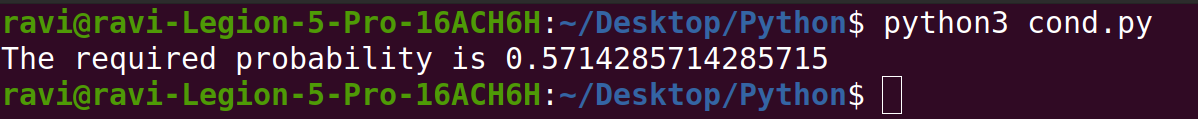
\includegraphics[width=\columnwidth]{../Figures/cond.png}
  \end{figure}
\end{frame}


\end{document}
